\setcounter{section}{0}
\section{HÀM SỐ VÀ ĐỒ THỊ}
\subsection{TÓM TẮT LÝ THUYẾT}
\subsubsection{Khái niệm hàm số. Tập xác định và tập giá trị của hàm số}
\begin{itemize}
	\item [\faSunO] \textbf{Định nghĩa:} Giả sử $x$ và $y$ là hai đại lượng biến thiên và $x$ nhận giá trị thuộc tập số $\mathscr{D}$.	Nếu với \textbf{mỗi giá trị $x$ thuộc $\mathscr{D}$}, ta xác định được \textbf{một và chỉ một giá trị tương ứng $y$} thuộc tập hợp số thực $\mathbb{R}$ thì ta có một hàm số.
	\begin{khung}
		\begin{itemize}
			\item Ta gọi $x$ là biến số và $y$ là hàm số của $x$.
			\item Tập hợp $\mathscr{D}$ được gọi là tập xác định của hàm số.
			\item Tập hợp $T$ gồm tất cả các giá trị $y$ (tương ứng với $x$ thuộc $\mathscr{D}$) gọi là tập giá trị của hàm số.
		\end{itemize}
	\end{khung}
	\item [\faSunO] \textbf{Cách cho một hàm số:} Một hàm số có thể được cho bởi một công thức hoặc nhiều công thức; có thể cho bằng mô tả; cho bằng bảng hoặc cho bằng biểu đồ.
\end{itemize}
% \begin{vd}
% 	Bản tin dự báo thời tiết cho biết nhiệt độ ở một số thời điểm trong ngày 01/05/2021 tại thành phố Hồ Chí Minh được ghi lại với biểu đồ bên dưới\\
% 	\centerline{\begin{tikzpicture}[font=\footnotesize, x=1.2cm,line join=round, line cap=round, >=stealth,scale=0.7,color=cyan]
% 		\draw[->] (.5,0)--(.5,5.5)node[left]{nhiệt độ};
% 		\draw[->] (.5,0)--(9,0) node[below]{giờ};
% 		\foreach \x/\y in {0/24,1/26,2/28,3/30,4/32,5/34} {
% 			\draw (.5,\x) node[left]{$\y$};}
% 		\foreach \x/\y in {1/1,2/4,3/7,4/10,5/13,6/16,7/19,8/22}\draw (\x,0.1)--(\x,-0.1) node [below] {\footnotesize $\y$};
% 		\foreach \x in {1,2,...,5} { \draw[orange!30] (.5,\x)--(9,\x); }
% 		\draw [line width=1pt,blue] (1,2)node[above]{\scriptsize $28$}--(2,1.5)node[above]{\scriptsize $27$}--(3,2)node[above left]{\scriptsize $28$}--(4,4)node[above]{\scriptsize $32$}--(5,3.5)node[above]{\scriptsize $31$}--(6,2.5)node[above]{\scriptsize $29$}--(7,2)node[above]{\scriptsize $28$}--(8,1.5)node[above]{\scriptsize $27$};
% 	\end{tikzpicture}}\\
% Rõ ràng với mỗi mốc giờ xác định trong ngày, ta có tương ứng duy nhất 1 số đo nhiệt độ được dự báo nên  có xem đây là 1 hàm số với
% 	\begin{itemize}
% 		\item  Tập xác định $D=\{1;4;7;10;13;16;19;22\}$
% 		\item  Tập giá trị $T=\{28; 27; 32;31;29\}$.
% 	\end{itemize}
% \end{vd}
% \begin{vd}
% 	Xét công thức $y=2x+1$. Ta đã biết đây là một hàm số bậc nhất với
% 	\begin{itemize}
% 		\item  Tập xác định $D=\mathbb{R}$
% 		\item  Tập giá trị $T=\mathbb{R}$.
% 	\end{itemize}
% \end{vd}
\subsubsection{Đồ thị hàm số}
\begin{itemize}
	\item [\faSunO] \textbf{Định nghĩa:} Cho hàm số $y=f(x)$ có tập xác định $\mathscr{D}$. Trên mặt phẳng toạ độ $Oxy$, đồ thị $(C)$ của hàm số là tập hợp tất cả các điểm $M(x;y)$ với $x \in \mathscr{D}$ và $y=f(x)$. Vậy $(C)=\{M(x;f(x)) \mid x \in \mathscr{D}\}$.
	\item [\faSunO] \textbf{Lưu ý:} Điểm $M\left(x_{M};y_{M}\right)$ thuộc đồ thị hàm số $y=f(x)$ khi và chỉ khi $x_{M} \in \mathscr{D}$ và $y_{M}=f\left(x_{M}\right)$.
\end{itemize}
\subsubsection{Sự đồng biến, hàm số nghịch biến của hàm số}
\begin{itemize}
	\item [\faSunO] \textbf{Khái niệm:} Với hàm số $y=f(x)$ xác định trên khoảng $(a;b)$, ta nói
	\begin{itemize}
		\item [\iconCH] Hàm số đồng biến trên khoảng $(a;b)$ nếu
		\boxmini{$\forall x_{1}, x_{2} \in(a ; b), x_{1}<x_{2} \Rightarrow f\left(x_{1}\right)<f\left(x_{2}\right)$}
		\item [\iconCH] Hàm số nghịch biến trên khoảng $(a;b)$ nếu
		\boxmini{$\forall x_{1}, x_{2} \in(a ; b), x_{1}<x_{2} \Rightarrow f\left(x_{1}\right)>f\left(x_{2}\right)$}
	\end{itemize}
	\item [\faSunO] \textbf{Lưu ý:} Khi vẽ bảng biến thiên, xét từ trái sang phải, ta dùng mũi tên đi xuống để minh họa khoảng nghịch biến và mũi tên đi lên để minh họa khoảng đồng biến. 
\end{itemize}

\subsection{RÈN LUYỆN KĨ NĂNG GIẢI TOÁN}
\begin{dang}{Tính giá trị của hàm số tại một điểm}
	Cho hàm số $y=f(x)$ có tập xác định $\mathscr{D}$ và $x_0 \in \mathscr{D}$.
	\begin{itemize}
		\item[\faPencilSquareO] Tính giá trị hàm số tại $x_0$: Ta chỉ việc thay $x_0$ vào biểu thức $y=f(x)$, tìm được $y_0$.
		\item[\faPencilSquareO] Nếu $f(x)$ là hàm cho bởi nhiều biểu thức thì ta thay $x_0$ vào biểu thức mà miền xác định của nó chứa $x_0$.
	\end{itemize}
\end{dang}

\begin{vd}
	Cho hai hàm số $f(x)=x^2-2x$ và $g(x)=1-x$. Tính $f(1)$; $g(-2)$; $f(1)+g(-2)$.
	\loigiai{}
\end{vd}

\begin{vd}
	Cho hàm số $f(x)=\heva{&3x-2 &\text{với } &x\ge 1 \\&1-2x^2 &\text{với } &x<1}$. Tính $f(1), f(2), f(0), f(-3)$.
		\loigiai{}
\end{vd}



\begin{vd}
	Cho hàm số $y=2x^3-3(m-1)x+2$, với $m$ là tham số. 
	\begin{tasks}
		\task Tìm $m$ để đồ thị hàm số đi qua điểm $M(1;2)$.
		\task Tìm $m$ để đồ thị hàm số đi qua điểm $N(-3;1)$.
	\end{tasks}
	\loigiai{}
\end{vd}

\begin{vd}
\immini{ Cho hàm số $y=f(x)$ và hàm số $y=g(x)$ có đồ thị như hình bên.
	\begin{tasks}
		\task Trong các điểm $A(2;2)$ $B(4;2)$, $C(3;3)$ điểm nào thuộc đồ thị $f(x)$? điểm nào thuộc đồ thị $g(x)$?
		\task Tính giá trị $f(1)+g(2)$.
		\task Tìm điểm trên đồ thị $f(x)$ có tung độ bằng $3$.
	\end{tasks}
}{
	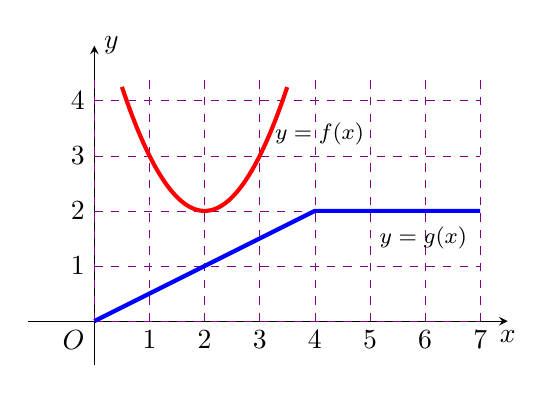
\begin{tikzpicture}[>=stealth,scale=0.7]
	\draw[->] (-1.2,0)--(0,0)%
	node[below left]{$O$}--(7.5,0) node[below]{$x$};
	\draw[->] (0,-0.8) --(0,5) node[right]{$y$};
	\foreach \x in {1,2,3,4,5,6,7}{
		\draw (\x,0) node[below]{$\x$};%Ox
	}
	\foreach \y in {1,2,3,4}{
		\draw (0,\y) node[left]{$\y$};%Oy
	}
	\draw[violet,dashed,line width=0.2pt] (0,0) grid (7,4.5);
	\draw [blue, line width=1.5pt] (0,0)--(4,2)--(7,2);
	\draw [red, line width=1.5pt, domain=0.5:3.5, samples=100] %
	plot (\x, {(\x)^2 -4*(\x)+6});
	\draw (3.1,3.4)node[right]{\footnotesize$y=f(x)$} (5,1.5)node[right]{\footnotesize $y=g(x)$};
	
	\end{tikzpicture}}
	\loigiai{}
\end{vd}

\begin{dang}{Tìm tập xác định, tập giá trị của hàm số}
	\begin{itemize}
		\item [\faSunO] \textbf{Tập xác định:} Ta tìm tập hợp tất cả các giá trị của $x$ để hàm số đã cho có nghĩa. Cần lưu ý hai vấn đề sau:
		\begin{listEX}[2]
			\item [\ding{172}] $\dfrac{A}{B}$ có nghĩa khi $B \ne 0$.
			\item [\ding{173}] $\sqrt{B}$ có nghĩa khi $B \ge 0$.
		\end{listEX}
		\item [\faSunO] \textbf{Tập giá trị:} Với $x$ thuộc miền xác định $\mathscr{D}$, ta có thể căn cứ vào bảng biến thiên hoặc đồ thị để tìm miền giá trị (\textit{nhìn khoảng "dao động" của} $y$.).
	\end{itemize}

\end{dang}

\begin{vd}%[0D2B1-1]
	Sau khi đun nóng băng phiến lên đến gần $90^{\circ}C$, người ta để nguội, quan sát, ghi nhận nhiệt độ và trạng thái của băng phiến sau mẫu phút như bảng sau
	\begin{center}
	\textit{Nhiệt độ và trạng thái của băng phiến khi để nguội}
		\begin{tabular}{|l|c|c|c|c|c|c|c|c|c|c|c|}
			\hline 
			\textbf{Thời gian nguội (phút)} & $0$ & $1$ & $2$ & $3$ & $4$ & $5$ & $6$ & $7$ & $8$ & $9$ & $10$ \\ 
			\hline 
			\textbf{Nhiệt độ ($^{\circ}C$)} & $86$ & $84$ & $82$ & $81$ & $80$ & $80$ & $80$  &$80$ & $79$ & $77$ & $75$ \\
			\hline
			\textbf{Trạng thái} & \multicolumn{4}{|c|}{lỏng} &\multicolumn{4}{|c|}{lỏng và rắng} & \multicolumn{3}{|c|}{rắn}\\
			\hline
		\end{tabular}
	\end{center}
\begin{tasks}(1)
	\task Tại sao từ bảng trên, có thể nói nhiệt độ của băng phiến là một hàm số theo thời gian (nung nóng)? Tìm tập xác định và tập giá trị của hàm số trên.
	\task Sau khi để nguội $3$ phút, nhiệt độ băng phiến là bao nhiêu?
	\task Băng phiến chuyển hoàn toàn sang trạng thái rắn sau bao nhiêu phút?
\end{tasks}
	\loigiai{
		\begin{enumerate}[a)]
			\item Bảng giá trị cho thấy nhiệt độ (kí hiệu là $y$) là một hàm số theo thời gian (kí hiệu là $x$) vì khi cho $x$ một giá trị bất kì, ta luôn tìm được duy nhất một giá trị của $y$. Do vậy bảng này xác định một hàm số biểu thị nhiệt độ của băng phiến theo thời gian.\\
			Từ bảng giá trị của hàm số, ta có tập xác định $\mathscr{D}=\{0 ; 1 ; 2 ; 3 ; 4 ; 5 ; 6 ; 7 ; 8 ; 9 ; 10\}$ và tập giá trị $T=\{75 ; 77 ; 79 ; 80 ; 81 ; 82 ; 84 ; 86\}$.
			\item Sau khi để nguội $3$ phút, nhiệt độ băng phiến là $81^{\circ}C$.
			\item Băng phiến chuyển hoàn toàn sang trạng thái rắn sau $8$ phút (lúc đó nhiệt độ băng phiến là $79^{\circ}$).
		\end{enumerate}
	}
\end{vd}

\begin{vd}
	\immini{Cho hàm số $y=f(x)$ có tập xác định là $\mathscr{D}$ và đồ thị là đường liền nét được vẽ trên miền $\mathscr{D}$ như hình bên
	\begin{tasks}(1)
		\task Xác định tập xác định $\mathscr{D}$.
		\task Tìm tập giá trị của hàm số trên miền $\mathscr{D}$.
		\task Tìm các điểm thuộc đồ thị và có tung độ bằng $3$.
	\end{tasks}}{
	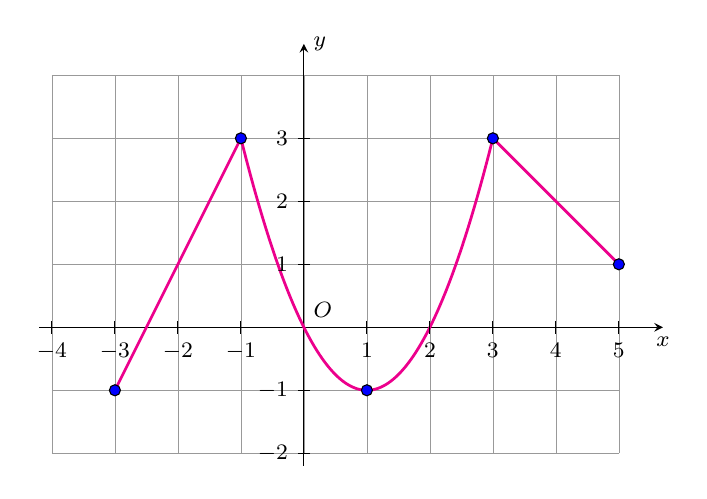
\begin{tikzpicture}[smooth,samples=300,scale=0.8,>=stealth,font=\footnotesize]
		\draw[line width=0.1pt,gray!80] (-4,-2) grid (5,4);
		\draw[->] (-4.2,0)--(5.7,0) node[below]{$x$};
		\draw[->] (0,-2.2)--(0,4.5) node[right]{$y$};
		\draw (0,0) node[above right]{$O$};
		\draw[line width=1pt,domain=-1:3,magenta] plot(\x,{(\x-1)^2-1});
		\draw[line width=1pt,magenta] (-3,-1)--(-1,3) (3,3)--(5,1);
		\draw[fill=blue] (-3,-1) circle(2.5pt) (-1,3) circle(2.5pt) (3,3) circle(2.5pt) (5,1) circle(2.5pt) (1,-1) circle(2.5pt);
		\foreach \x in {-4,-3,-2,-1,1,2,3,4,5}\draw (\x,0.1)--(\x,-0.1) node [below] {\footnotesize $\x$};
		\foreach \y in {-2,-1,1,2,3}\draw (0.1,\y)--(-0.1,\y) node [left] {\footnotesize $\y$};
\end{tikzpicture}}
	\loigiai{}
\end{vd}

\begin{vd}
	Tìm tập xác định của các hàm số sau đây:
	\begin{listEX}[2]
		\item $y=x^4+x^2-2$.
		\item $y=\dfrac{x+2}{x-2}$.
		\item $y=\dfrac{x^2+2}{4-x}$.
		\item $y=\dfrac{1}{-x^2+3x}$
	\end{listEX}
	\loigiai{}
\end{vd}
\begin{vd}
	Tìm tập xác định của các hàm số sau đây:
	\begin{listEX}[2]
		\item $y=\sqrt{x-2}$.
		\item $y=\dfrac{2x-1}{\sqrt{x+2}}$.
		\item $y=x+\dfrac{1}{\sqrt{3-x}}$.
		\item $y=\sqrt{2+x}+\sqrt{x-2}$.
	\end{listEX}
	\loigiai{}
\end{vd}

\begin{vd}
	Tìm tập xác định của các hàm số sau:
	\begin{listEX}[2]
		\item $f(x)=\heva{&2x+1 &\text{ nếu }& x \le 0 \\& x^2 &\text{ nếu }& x > 0}$.
		\item $f(x)=\heva{&\dfrac{1}{x-1}&\text{ nếu }& x \le 2 \\& x^2 &\text{ nếu }& x > 2}$.
	\end{listEX}
\loigiai{
	\begin{enumerate}[a)]
		\item Ta xét hai trường hợp
		\begin{itemize}
			\item [$\bullet$] Khi $x\le 0$ thì $f(x)=2x+1$. Hàm này luôn xác định với mọi $x \in \mathbb{R}$ nên sẽ xác định với mọi $x \le 0$.
			\item [$\bullet$] Khi $x>0$ thì $f(x)=x^2$. Hàm này luôn xác định với mọi $x\in \mathbb{R}$ nên sẽ xác định với mọi $x >0$.
		\end{itemize}
	Kết hợp hai trường hợp, ta được tập xác định của hàm số là $\mathscr{D}=\mathbb{R}$.
		\item Ta xét hai trường hợp
		\begin{itemize}
			\item [$\bullet$] Khi $x\le 2$ thì $f(x)=\dfrac{1}{x-1}$. Hàm này  xác định khi và chỉ khi $x-1 \ne 0 \Leftrightarrow x \ne 1$.
			\item [$\bullet$] Khi $x>2$ thì $f(x)=x^2$. Hàm này luôn xác định với mọi $x\in \mathbb{R}$ nên sẽ xác định với mọi $x >2$.
		\end{itemize}
		Kết hợp hai trường hợp, ta được tập xác định của hàm số là $\mathscr{D}=\mathbb{R}\backslash \{1\}$.
\end{enumerate}}
\end{vd}


\begin{dang}{Tìm khoảng đồng biến, khoảng nghịch biến của hàm số}
\begin{itemize}
	\item[\faPencilSquareO] Nếu đề bài cho bảng biến thiên hoặc đồ thị: Xét từ trái sang phải thì
	\begin{itemize}
		\item [$\bullet$] Khoảng nào có mũi tên đi xuống (đồ thị đổ xuống) thì khoảng đó hàm số nghịch biến.
		\item [$\bullet$] Khoảng nào có mũi tên đi lên (đồ thị đi lên) thì khoảng đó hàm số đồng biến.
	\end{itemize}
	\item[\faPencilSquareO] Nếu đề bài yêu cầu xét tính đồng biến, nghịch biến của hàm số $y=f(x)$ trên khoảng xác định $(a;b)$:  Ta lấy $x_1, x_2$ tùy ý thuộc $(a;b)$, với $x_1<x_2$ và tính $f(x_1)-f(x_2)$, nếu
	\begin{itemize}
		\item [$\bullet$] $f(x_1)-f(x_2)<0$ thì hàm số $y=f(x)$ đồng biến trên khoảng $(a;b)$.
		\item [$\bullet$] $f(x_1)-f(x_2)>0$ thì hàm số $y=f(x)$ nghịch biến trên khoảng $(a;b)$.
	\end{itemize}
	\item[\faPencilSquareO] Trong nhiều trường hợp, để tìm được khoảng đồng biến và nghịch biến của hàm số, ta có thể lập bảng biến thiên của hàm số đó trên miền xác định.
\end{itemize}
\end{dang}
\begin{vd}
	\immini{Cho hàm số $y=f(x)$ có tập xác định là $\mathscr{D}$ và đồ thị là đường liền nét được vẽ trên miền $\mathscr{D}$ như hình bên. Tìm các khoảng đồng biến và nghịch biến của hàm số trên miền $\mathscr{D}$.
	}{
		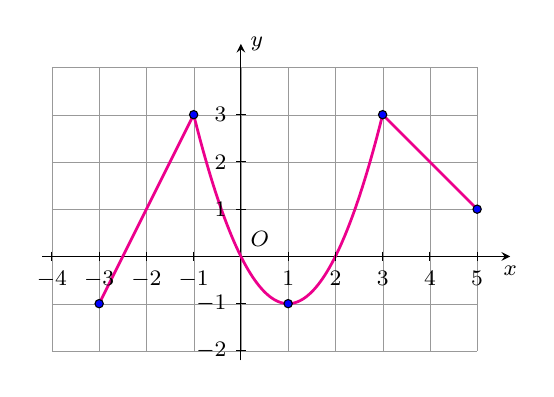
\begin{tikzpicture}[smooth,samples=300,scale=0.6,>=stealth,font=\footnotesize]
			\draw[line width=0.1pt,gray!80] (-4,-2) grid (5,4);
			\draw[->] (-4.2,0)--(5.7,0) node[below]{$x$};
			\draw[->] (0,-2.2)--(0,4.5) node[right]{$y$};
			\draw (0,0) node[above right]{$O$};
			\draw[line width=1pt,domain=-1:3,magenta] plot(\x,{(\x-1)^2-1});
			\draw[line width=1pt,magenta] (-3,-1)--(-1,3) (3,3)--(5,1);
			\draw[fill=blue] (-3,-1) circle(2.5pt) (-1,3) circle(2.5pt) (3,3) circle(2.5pt) (5,1) circle(2.5pt) (1,-1) circle(2.5pt);
			\foreach \x in {-4,-3,-2,-1,1,2,3,4,5}\draw (\x,0.1)--(\x,-0.1) node [below] {\footnotesize $\x$};
			\foreach \y in {-2,-1,1,2,3}\draw (0.1,\y)--(-0.1,\y) node [left] {\footnotesize $\y$};
	\end{tikzpicture}}
	\loigiai{}
\end{vd}
\begin{vd}
	Cho hàm số $y=f(x)=-2x^2-7$. Xét tính đồng biến và nghịch biến của hàm số trên các khoảng $(-4;0)$; $(3;10)$.
		\loigiai{}
\end{vd}


\begin{vd}
	Xét tính đồng biến và nghịch biến của hàm số $y=f(x)=x^2+10x+9$ trên $(-5;+\infty)$.
		\loigiai{}
\end{vd}

\begin{vd}
	Xét tính đồng biến và nghịch biến của hàm số $y=f(x)=\dfrac{x}{x-7}$ trên các khoảng $(-\infty;7)$;  $(7;+\infty)$.
		\loigiai{}
\end{vd}

\begin{dang}{Vẽ đồ thị hàm số cho bởi nhiều biểu thức}
	
\end{dang}
\begin{vd}
	Tìm tập xác định và vẽ đồ thị các hàm số sau:
	\begin{tasks}(2)
		\task $f(x)=\heva{& 2x & \text{ với }& x \ge 0 \\ & -x & \text{ với }& x<0.}$
		\task $f(x)=\heva{& -x^2 & \text{ với }& x\le 1\\ & 1 & \text{ với }& x>1.}$
		\task $f(x)= \big|x\big|$.
		\task $f(x)= \big|x+2\big|$.
	\end{tasks}
	\loigiai{}
\end{vd}


\begin{dang}{Viết công thức hàm số cho một số bài toán thực tế}
\end{dang}

\begin{vd}%[0D2T1-1]
	Theo quyết định số 2019/QĐ-BĐVN ngày 01/11/2018 của Tổng công ty Bưu điện Việt Nam, giá cước dịch vụ Bưu chính phổ cập đối với dịch vụ thư cơ bản và bưu thiếp trong nước có khối lượng đến $250$g như trong bảng sau
	\immini{\begin{enumerate}[a)]
			\item Số tiền dịch vụ thư cơ bản phải trả $y$ (đồng) có là hàm số của khối lượng thư cơ bản $x$ (g) hay không? Nếu đúng, hãy xác định những công thức tính $y$.
			\item Tính số tiền phải trả khi bạn Dương gửi thư có khối lượng $150$g, $200$g.
	\end{enumerate} }
	{\vspace{0.6 cm}
		\begin{tabular}{|c|c|}
			\hline
			\textcolor{blue}{Khối lượng đến $250$ g} & \textcolor{blue}{Mức cước (đồng)}\\
			\hline
			Đến $20$ g & $4000$\\
			\hline
			Trên $20$ g đến $100$ g & $6000$ \\
			\hline
			Trên $100$ g đến $250$ g & $8000$\\
			\hline
	\end{tabular}}
	\loigiai{
		\begin{enumerate}[a)]
			\item Số tiền dịch vụ thư cơ bản phải trả $y$ là hàm số của $x$ vì mỗi giá trị của $x$ (chính là khối lượng của thư) có đúng một giá trị của $y$ (mức cước hay số tiền phải trả) tương ứng.\\
			Quan sát bảng ta thấy:
			\begin{itemize}
				\item[$\bullet$] Nếu khối lượng thư đến $20$ g hay $0<x \le 20$ thì mức cước phải trả là $4000$ đồng hay $y= 4000$.
				\item[$\bullet$] Nếu khối lượng thư trên $20$ g hay $100$ g hay $20 < x \le 100$ g thì mức cước là $6000$ đồng hay $y=6000$.
				\item[$\bullet$] Nếu khối lượng thư trên $100$ g đến $250$ g hay $100 < x \le 250$ thì mức cước là $8000$ đồng hay $y=8000$.
			\end{itemize}
			Vậy ta có công thức xác định $y$ như sau:
			$y=\heva{&4000&\text{nếu}& 0<x\le 20\\&6000&\text{nếu}& 20 <x\le 100\\&8000&\text{nếu}& 100<x\le 250.}$
			\item Vì $100 < 150 <250$ và $100 <200 <250$ nên bức thư có khối lượng $150$ g thì cần trả cước là $8000$ đồng và bức thư có khối lượng $200$ g cũng cần trả cước là $8000 $ đồng. \\
			Vậy tổng số tiền phải trả khi bạn Dương gửi thư có khối lượng $150$ g và $200$ g là \\ \centerline{$8000 + 8000 = 16 000$ (đồng).}
		\end{enumerate}
	}
\end{vd}


\begin{vd}
	Nhiệt độ ở mặt đất đo được khoảng $30^{\circ} \mathrm{C}$. Biết rằng cứ lên $1 \mathrm{~km}$ thì nhiệt độ giảm đi $5^{\circ}$.
	\begin{tasks}(1)
		\task Hãy lập hàm số $T$ theo $h$, trong đó $T$ tính bằng độ $\left({ }^{\circ}\right)$ và $h$ tính bằng ki-lô-mét $(\mathrm{km})$.
		\task Hãy tính nhiệt độ khi ở độ cao $3 \mathrm{~km}$ so với mặt đất.
	\end{tasks}
	\loigiai{
		\begin{enumerate}[a)]
			\item Hàm số $T$ theo $h$ là $T=30-5h$.
			\item Thay $h=3$ vào công thức $T=30-5h$, ta được $
			T=30-5 \cdot 3=15$.\\
			Vậy khi lên độ cao $3 \mathrm{~km}$ thì nhiệt độ tại đó là $15^{\circ}$
	\end{enumerate}}
\end{vd}

\begin{vd}%[0D2T1-1]
	Một công ty viễn thông A cung cấp dịch vụ truyền hình cáp với mức phí ban đầu là 300000 đồng và mỗi tháng phải đóng 150000 đồng. Công ty viễn thông B cũng cung cấp dịch vụ truyền hình cáp nhưng không tính phí ban đầu và mỗi tháng khách hàng sẽ phải đóng 200000 đồng.
	\begin{tasks}(1)
		\task Gọi $T$ (đồng) là số tiền khách hàng phải trả cho mỗi công ty viễn thông trong $t$ (tháng) sử dụng dịch vụ truyền hình cáp. Khi đó hãy lập hàm số $T$ theo $t$ đối với mỗi công ty.
		\task Tính số tiền khách hàng phải trả sau khi sử dụng dịch vụ truyền hình cáp trong 5 tháng đối với mỗi công ty.
		\task Khách hàng cần sử dụng dịch vụ truyền hình cáp trên mấy tháng thì đăng kí bên công ty viễn thông A sẽ tiết kiệm chi phí hơn?
	\end{tasks}
	\loigiai{
		\begin{enumerate}[a)]
			\item Hàm số $T$ theo $t$ đối với công ty A là $T=150000t+300000$.\\
			Hàm số $T$ theo $t$ đối với công ty B là $T=200000t$.
			\item Thay $t=5$ lần lượt vào hai công thức trên, ta được
			\begin{itemize}
				\item [$\bullet$] Số tiền phải trả trong 5 tháng khi sử dụng dịch vụ truyền hình cáp của công ty A là $150000.5+300000=1050000$ đồng.
				\item [$\bullet$] Số tiền phải trả trong 5 tháng khi sử dụng dịch vụ truyền hình cáp của công ty B là $200000.5=1000000$ đồng.
			\end{itemize}
			\item Để dịch vụ truyền hình cáp của công ty A lợi hơn dịch vụ truyền hình cáp của công ty B thì:
			$$
			150000t+300000<200000t \Leftrightarrow 300000<50000t \Leftrightarrow t>6
			$$
			Vậy nếu sử dụng từ 7 tháng trở lên thì sử dụng dịch vụ truyền hình cáp bên công ty A sẽ có lợi hơn.
	\end{enumerate}}
\end{vd}
\subsection{BÀI TẬP TỰ LUYỆN}

\begin{bt}%[0D2T1-1]
	Trong kinh tế thị trường, lượng cầu và lượng cung là hai khái niệm quan trọng. Lượng cầu chỉ khả năng về số lượng sản phẩm cần mua của bên mua (người tiêu dùng), tuỳ theo đơn giá bán sản phẩm; còn lượng cung chỉ khả năng cung cấp số lượng sản phẩm nảy cho thị trường của bên bán (nhà sản xuất) cũng phụ thuộc vào đơn giá bán sản phẩm.\\
	Người ta khảo sát nhu cầu của thị trường đối với sản phẩm $\mathrm{A}$ theo đơn giá của sản phẩm này và thu được bảng sau:
	\begin{center}
		\begin{tabular}{|c|c|c|c|c|c|}
			\hline Đơn giá sản phẩm $A$ (đơn vị: nghìn đồng) & 10 & 20 & 40 & 70 & 90 \\
			\hline Lượng cầu (nhu cầu về số sản phẩm) & 338 & 288 & 200 & 98 & 50 \\
			\hline
		\end{tabular}
	\end{center}
	\begin{enumerate}
		\item Hãy cho biết tại sao bảng giá trị trên xác định một hàm số? Hãy tìm tập xác định và tập giá trị của hàm số đó (gọi là hàm cầu).
		\item Giả sử lượng cung của sản phẩm $A$ tuân theo công thức $y=f(x)=\dfrac{x^{2}}{50}$, trong đó $x$ là đơn giá sản phẩm $A$ và $y$ là lượng cung ứng với đơn giá này. Hãy điền các giá trị của hàm số $f(x)$ (gọi là hàm cung) vào bảng sau
		\begin{center}
			\begin{tabular}{|c|l|l|l|l|l|}
				\hline Đơn giá sản phẩm $A$ (đơn vị: nghìn đồng) & 10 & 20 & 40 & 70 & 90 \\
				\hline Lượng cung (khả năng cung cấp về số sản phẩm) & & & & & \\
				\hline
			\end{tabular}
		\end{center}
		\item Ta nói thị trường của một sản phẩm là cần bằng khi lượng cung và lượng cầu bằng nhau. Hãy tìm đơn giá $x$ của sản phẩm $A$ khi thị trường cân bằng.
	\end{enumerate}
	\loigiai{
		\begin{enumerate}
			\item Có thể thấy với mỗi mức đơn giá, đều có duy nhất một giá trị về lượng cầu. Do vậy, bảng giá trị đã cho ở đề bài xác định một hàm số.\\
			Hàm số có tập xác định $\mathscr{D}=\{10;20;40;70;90\}$ và tập giá trị $\mathscr{T}=\{338;288;200;98;50\}$.\\
			\item \hfill
			\begin{center}
				\begin{tabular}{|c|c|c|c|c|c|}
					\hline Đơn giá sản phẩm $A$ (đơn vị nghìn đồng) & 10 & 20 & 40 & 70 & 90 \\
					\hline Lượng cung (khả năng cung cấp về số sản phẩm) & 2 & 8 & 32 & 98 & 162 \\
					\hline
				\end{tabular}
			\end{center}
			\item Dựa vào hai bảng giá trị của lượng cung và lượng cầu, ta tìm được giá trị $x=70$ thì lượng cung và lượng cầu đều bằng $98$.\\
			Vậy thị trường của sản phẩm $A$ cân bằng khi đơn giá của sản phẩm $\mathrm{A}$ này là $70\,000$(đồng).
		\end{enumerate}
	}
\end{bt}

\begin{bt}
	\immini{Cho hàm số $y=f(x)$ có tập xác định là $\mathscr{D}$ và đồ thị là đường liền nét được vẽ trên miền $\mathscr{D}$ như hình bên. 
		\begin{tasks}(1)
			\task Trong các điểm $A(2;2)$, $B(0;1)$, $C(4;2)$, $D(-3;-1)$, điểm nào thuộc $(C)$? điểm nào không thuộc $(C)$?
			\task Tìm tập xác định $\mathscr{D}$ và tập giá trị $\mathscr{T}$ của hàm số  $y=f(x)$. 
			\task Tìm các khoảng đồng biến và nghịch biến của hàm số trên miền $\mathscr{D}$.
		\end{tasks}
		
	}{
		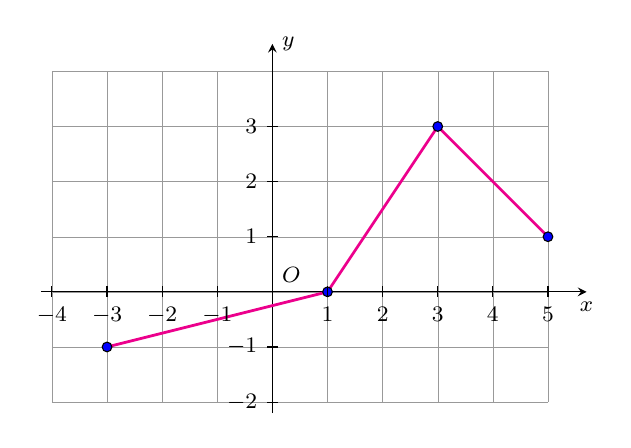
\begin{tikzpicture}[smooth,samples=300,scale=0.7,>=stealth,font=\footnotesize]
			\draw[line width=0.1pt,gray!80] (-4,-2) grid (5,4);
			\draw[->] (-4.2,0)--(5.7,0) node[below]{$x$};
			\draw[->] (0,-2.2)--(0,4.5) node[right]{$y$};
			\draw (0,0) node[above right]{$O$};
			\draw[line width=1pt,magenta] (-3,-1)--(1,0)-- (3,3)--(5,1);
			\draw[fill=blue] (-3,-1) circle(2.5pt) (1,0) circle(2.5pt) (3,3) circle(2.5pt) (5,1) circle(2.5pt);
			\foreach \x in {-4,-3,-2,-1,1,2,3,4,5}\draw (\x,0.1)--(\x,-0.1) node [below] {\footnotesize $\x$};
			\foreach \y in {-2,-1,1,2,3}\draw (0.1,\y)--(-0.1,\y) node [left] {\footnotesize $\y$};
	\end{tikzpicture}}
	\loigiai{}
\end{bt}

\begin{bt}
	Cho hai hàm số $f(x)=x^2-2x$ và $g(x)=1-\sqrt{x}$. Tính giá trị $\dfrac{f(-1)}{g(4)}$.
		\loigiai{}
\end{bt}

\begin{bt}
	Cho hàm số $f(x)=4-\sqrt[3]{x}$.
	\begin{listEX}[3]
		\item Tính $f(-8)$.
		\item Tính $f(a^3)$.
		\item Tìm $a>0$ thỏa $f(a^6)=0$
	\end{listEX}
	\loigiai{}
\end{bt}

\begin{bt}
	Cho hàm số $f(x)=\heva{&x^2-2x-1 &\text{với } x\le 0 \\&\dfrac{x+1}{x^2+x+1} &\text{với } x > 0}$. Tính giá trị của hàm số đó tại $x=1; x=0; x=-2$.
		\loigiai{}
\end{bt}

\begin{bt}%[0D2B1-2]
	Tìm tập xác định của mỗi hàm số sau
	\begin{tasks}(2)
		\task $y=-x^2$.
		\task $y = \sqrt{2-3x}$.
		\task $y = \dfrac{4}{x+1}$.
		\task $y = \heva{& 1 &\text{ nếu }& x \in \mathbb{Q} \\ & 0 &\text{ nếu }& x \in \mathbb{R} \setminus \mathbb{Q}.}$
	\end{tasks}
	\loigiai{
		\begin{enumerate}[a)]
			\item Hàm số $y = -x^2$ có tập xác định $\mathscr{D} = \mathbb{R}$.
			\item Biểu thức $\sqrt{2-3x}$ có nghĩa khi $2 - 3x \geq 0 \Leftrightarrow x \leq \dfrac{2}{3}$. \\
			Vậy tập xác định $\mathscr{D} = \left(-\infty;\dfrac{2}{3}\right]$.
			\item Biểu thức $\dfrac{4}{x+1}$ có nghĩa khi và chỉ khi $x \ne - 1$. \\
			Vậy tập xác định $\mathscr{D} = \mathbb{R} \setminus \{-1 \}$.
			\item Tập xác định $\mathscr{D} = \mathbb{R}$.
		\end{enumerate}
	}
\end{bt}

\begin{bt}%[0D2B1-2]%
	Tìm tập xác định của các hàm số sau
	\begin{tasks}(2)
		\task $y=2-4x$.
		\task $y=\dfrac{x-3}{5-2x}$.
		\task $y=\dfrac{x}{x^2-3x+2}$.
		\task $y=\dfrac{2x+1}{(x-2) \left( x^2-4x+3 \right)}$.
	\end{tasks}
	\loigiai{
		\begin{enumEX}{1}
			\item Ta có $\mathscr{D}=\mathbb{R}$.
			\item Hàm số xác định khi $5-2x \neq 0 \Leftrightarrow x \neq \dfrac{5}{2}$.\\
			Tập xác định $\mathscr{D}=\mathbb{R} \setminus \left\{ \dfrac{5}{2} \right\}$.
			\item Hàm số xác định khi $x^2-3x+2 \neq 0 \Leftrightarrow \heva{&x \neq 1 \\ & x \neq 2}$.\\
			Tập xác định $\mathscr{D}=\mathbb{R} \setminus \{1;2\}$.
			\item Hàm số xác định khi $(x-2) \left( x^2-4x+3 \right) \neq 0 \Leftrightarrow \heva{& x-2\neq 0\\& x^2-3x+2\neq 0} \Leftrightarrow \heva{& x \neq 1\\ & x \neq 2 \\ & x \neq 3}$.\\
			Tập xác định $\mathscr{D}=\mathbb{R} \setminus \{1;2;3\}$.
		\end{enumEX}
	}
\end{bt}

\begin{bt}%[0D2B1-2]%
	Tìm tập xác định của các hàm số
	\begin{tasks}(2)
		\task $ y= \dfrac{\sqrt{ 4-2x}}{x^2-6x+5}$.
		\task $ y= \sqrt{ \dfrac{x^2}{x-1}}$.
	\end{tasks}
	\loigiai{
		\begin{enumerate}[a)]
			\item Hàm số xác định $\Leftrightarrow \heva{& 4-2x \geq 0\\&x^2-6x+5 \neq 0} \Leftrightarrow \heva{& x\leq 2\\& x \neq 1\\&x \neq 5} \Leftrightarrow \heva{& x\leq 2\\&x\neq 1.}$\\
			Vậy tập xác định của hàm số là $\mathscr {D} = \left(-\infty ;2\right] \backslash \{1\}$.
			\item Hàm số xác định $\Leftrightarrow \heva{& x\neq 1\\& \dfrac{x^2}{x-1}\geq 0} \Leftrightarrow \hoac{&x=0\\&x >1.}$\\
			Vậy tập xác định của hàm số là $\mathscr {D} = \{0\} \cup (1;+\infty)$.
		\end{enumerate}
	}
\end{bt}

\begin{bt}%[0D2B1-2]
	Tìm tập xác định các hàm số sau
	\begin{tasks}(2)
		\task $f(x)=\dfrac{4x-1}{\sqrt{2x-5}}$.
		\task $f(x)=\heva{& \dfrac{1}{x-3} & \text{ với }& x\ge 0\\ & 1 & \text{ với }& x<0.}$
	\end{tasks}
	\loigiai{
		\begin{enumerate}[a)]
			\item Hàm số xác định khi và chỉ khi $2x-5>0\Leftrightarrow x>\dfrac{5}{2}$.\\
			Tập xác định $\mathscr{D}=\left(\dfrac{5}{2};+\infty\right)$.
			\item Với $x\ge 0$ thì $f(x)=\dfrac{1}{x-3}$, khi đó $f(x)$ xác định khi $x-3\ne 0\Leftrightarrow x\ne 3$.\\
			Với $x<0$, $f(x)=1$ luôn xác định và nhận giá trị bằng $1$.\\
			Vậy tập xác định $\mathscr{D}=\mathbb{R}\setminus \{3\}$.
		\end{enumerate}	
	}
\end{bt}

\begin{bt}%[0D2B1-3]
	Xét sự biến thiên của hàm số sau trên khoảng $(1;+\infty)$.
	\begin{listEX}[2]
		\item $y=\dfrac{3}{x-1}$.
		\item $y=x+\dfrac{1}{x}$.
	\end{listEX}
	\loigiai{
		\begin{enumerate}[a)]
			\item Với mọi $x_1,\,x_2\in(1;+\infty),\,\,x_1\ne{x_2}$ ta có
			\[f(x_2)-f(x_1)=\dfrac{3}{x_2-1}-\dfrac{3}{x_1-1}=\dfrac{3(x_1-x_2)}{(x_2-1)(x_1-1)}.\]
			Suy ra $\dfrac{f(x_2)-f(x_1)}{x_2-x_1}=-\dfrac{3}{(x_2-1)(x_1-1)}$.\\
			Vì $x_1> 1,\,\,x_2> 1\Rightarrow\dfrac{f(x_2)-f(x_1)}{x_2-x_1}< 0$ nên hàm số $ y=\dfrac{3}{x-1}$ nghịch biến trên khoảng $(1;+\infty)$.
			\item Với mọi $x_1,\,x_2\in(1;+\infty),\,x_1\ne{x_2}$ ta có
			\[f(x_2)-f(x_1)=\left(x_2+\dfrac{1}{x_2}\right)-\left(x_1+\dfrac{1}{x_1}\right)=(x_2-x_1)\left(1-\dfrac{1}{x_1x_2}\right).\]
			Suy ra $\dfrac{f(x_2)-f(x_1)}{x_2-x_1}=1-\dfrac{1}{x_1x_2}$.\\
			Vì $x_1> 1$, $x_2> 1\Rightarrow\dfrac{f(x_2)-f(x_1)}{x_2-x_1}> 0$.\\
			Vậy hàm số $ y=x+\dfrac{1}{x}$ đồng biến trên khoảng $(1;+\infty)$.
		\end{enumerate}
	}
\end{bt}


\begin{bt}%[0D2K1-3]
	Tìm khoảng đồng biến, nghịch biến của các hàm số sau
		\begin{listEX}[3]
			\item  $f(x)=1-3x$.
			\item  $f(x)=\dfrac{1}{x-3}$.
			\item   $f(x)=|2x-1|$.
		\end{listEX}
	\loigiai{
		\begin{enumerate}[a)]
			\item Hàm số có tập xác định $\mathscr{D}=\mathbb{R}$.\\
			Lấy $x_1$, $x_2$ là hai số tuỳ ý thỏa $x_1<x_2$ thì 
			$$f(x_1)-f(x_2)=-3(x_1-x_2)>0$$
			nên hàm số đã chi nghịch biến trên $\mathbb{R}$.
			\item Hàm số $f(x)=\dfrac{1}{x-3}$ xác định khi $x-3\ne 0\Leftrightarrow x\ne 3$\\
			Suy ra tập xác định $\mathscr{D}=\mathbb{R}\setminus \{3\}$.\\
			Lấy $x_1$, $x_2$ là hai số tuỳ ý cùng thuộc mỗi khoảng $(-\infty;3)$, $(3;+\infty)$ sao cho $x_1<x_2$, ta có
			$$f(x_1)-f(x_2)=\dfrac{1}{x_1-3}-\dfrac{1}{x_2-3}=\dfrac{x_2-x_1}{(x_1-3)(x_2-3)}.$$
			Do $x_1<x_2$ nên $x_2-x_1>0$.\\
			Mặt khác, khi lấy $x_1$ và $x_2$ cùng nhỏ hơn $3$ hoặc cùng lớn hơn $3$, ta đều có $x_1-3$ và $x_2-3$ luôn cùng dấu nên $(x_1-3)(x_2-3)<0$.\\
			Suy ra $f(x_1)-f(x_2)>0\Rightarrow f(x_1)>f(x_2)$.\\
			Vậy hàm số $f(x)$ luôn nghịch biến trên các khoảng $(-\infty;3)$ và $(3;+\infty)$.
			\item Hàm số $f(x)=|2x-1|$ còn được viết lại như sau
			$$f(x)=|2x-1|=\heva{& 2x-1 & \text{ với } 2x-1\ge 0\\ & -(2x-1)& \text{với } 2x-1<0}=\heva{& 2x-1 & \text{với }x\ge \dfrac{1}{2}\\ & -2x+1 & \text{với }x<\dfrac{1}{2}.}$$
			Xét hàm số $g(x)=2x-1$. Hàm số này xác định trên $\mathbb{R}$.\\
			Lấy hai số $x_1$, $x_2$ tuỳ ý sao cho $x_1<x_2$, ta có 
			$$x_1<x_2\Rightarrow 2x_1<2x_2\Rightarrow 2x_1-1<2x_2-1\Rightarrow g(x_1)<g(x_2).$$
			Suy ra $g(x)$ đồng biến trên $\mathbb{R}$ nên $f(x)$ đồng biến trên $\left(\dfrac{1}{2};+\infty\right)$.\\
			Xét hàm số $h(x)=-2x+1$. Hàm số này xác định trên $\mathbb{R}$.\\
			Lấy hai số $x_1$, $x_2$ tuỳ ý sao cho $x_1<x_2$, ta có 
			$$ x_1<x_2\Rightarrow -2x_1>-2x_2\Rightarrow -2x_1+1>-2x_2+1\Rightarrow h(x_1)>h(x_2).$$
			Suy ra $h(x)$ nghịch biến trên $\mathbb{R}$ nên $f(x)$ nghịch biến trên $\left(-\infty;\dfrac{1}{2}\right)$.\\
			Vậy hàm số $f(x)=|2x-1|$ đồng biến trên khoảng $\left(\dfrac{1}{2};+\infty\right)$ và nghịch biến trên khoảng $\left(-\infty;\dfrac{1}{2}\right)$.
			
		\end{enumerate}
	}
\end{bt}

\begin{bt}%[0D2B3-3]
	Vẽ đồ thị các hàm số sau
	\begin{tasks}(2)
		\task $f(x)=\heva{& x^2 & \text{ với }& x\le 2\\ & x+2 &\text{với }& x>2.}$
		\task $f(x)=|x+3|-2$.
	\end{tasks}
	\loigiai{
		\begin{enumerate}[a)]
			\item Ta vẽ đồ thị $g(x)=x^2$ và giữ phần đồ thị ứng với $x\le 2$, vẽ đồ thị $h(x)=x+2$ và giữ phần đồ thị ứng với $x>2$. Ta được đồ thị như hình vẽ
			\begin{center}
				\begin{tikzpicture}[scale=0.7, font=\footnotesize, line join=round, line cap=round,>=stealth]
					\def \xmin{-3};
					\def \xmax{6};
					\def \ymin{-1};
					\def \ymax{9};
					\draw[->] (\xmin, 0.) -- (\xmax,0.) node[anchor=north] {$x$};
					\draw[->] (0.,\ymin) -- (0.,\ymax) node[anchor=west] {$y$};
					\clip(\xmin-0.1,\ymin-0.1) rectangle (\xmax+0.1,\ymax+0.1);
					\draw[smooth] plot[domain=-3:2] (\x,{(\x)^2});
					\draw[dashed] plot[domain=2:3] (\x,{(\x)^2});
					\draw[smooth] plot[domain=2:6] (\x,{\x+2});
					\draw[dashed] plot[domain=-3:2] (\x,{\x+2});
					\foreach \i in {-2,-1,1,2,3,4,5}
					\draw[fill=black] (\i,0) circle(1pt) node[below]{$\i$};
					\foreach \j in {1,2,3,4,5,6,7,8}
					\draw[fill=black] (0,\j) circle(1pt) node[left]{$\j$};
					\draw[fill=black] (0,0) circle(1pt) node[below left]{$O$} (4,4) node[above]{$y=f(x)$} ;
					
				\end{tikzpicture}
			\end{center}
			\item Ta có $f(x)=|x+3|-2=\heva{& x+3-2 & \text{với } x+3\ge 0\\ & -(x+3)-2& \text{với }x+3<0}=\heva{& x+1& \text{với }x\ge -3\\ & -x-5& \text{với } x<-3.}$\\
			Ta vẽ đồ thị $g(x)=x+1$ và giữ lại phần đồ thị ứng với $x\ge -3$, đồng thời vẽ đồ thị $h(x)=-x-5$ và giữ lại phần đồ thị ứng với $x<-3$. Ta được đồ thị của $f(x)$ như sau
			\begin{center}
				\begin{tikzpicture}[scale=0.7, font=\footnotesize, line join=round, line cap=round,>=stealth]
					\def \xmin{-6};
					\def \xmax{2};
					\def \ymin{-5};
					\def \ymax{3};
					\draw[->] (\xmin, 0.) -- (\xmax,0.) node[anchor=north] {$x$};
					\draw[->] (0.,\ymin) -- (0.,\ymax) node[anchor=west] {$y$};
					\clip(\xmin-0.1,\ymin-0.1) rectangle (\xmax+0.1,\ymax+0.1);
					\draw[smooth] plot[domain=-3:2] (\x,{\x+1});
					\draw[dashed] plot[domain=-6:-3] (\x,{\x+1});
					\draw[smooth] plot[domain=-6:-3] (\x,{-\x-5});
					\draw[dashed] plot[domain=-3:2] (\x,{-\x-5});
					\foreach \i in {-5,-4,-3,-2,-1,1}
					\draw[fill=black] (\i,0) circle(1pt) node[below]{$\i$};
					\foreach \j in {1,2,-1,-2,-3,-4,-5}
					\draw[fill=black] (0,\j) circle(1pt) node[left]{$\j$};
					\draw[fill=black] (0,0) circle(1pt) node[below left]{$O$} (1,1) node[below]{$y=f(x)$} (-3,-2) circle(1pt);
					
				\end{tikzpicture}
			\end{center}
		\end{enumerate}
	}
\end{bt}

\begin{bt}%[0D2T1-1]
	Một lớp muốn thuê một chiếc xe khách cho chuyến tham quan với tổng đoạn đường cần di chuyển trong khoảng từ $550$ km đến $600$ km, có hai công ty được tiếp cận để tham khảo giá. Công ty A có giá khởi đầu là $3{,}75$ triệu đồng cộng thêm $5000$ đồng cho mỗi km chạy xe. Công ty B có giá khởi đầu là $2{,}5$ triệu đồng cộng thêm $7500$ đồng cho mỗi km chạy xe. Lớp đó nên chọn công ty nào để chi phí là thấp nhất?
	\loigiai{
		Hàm số biểu thị giá tiền theo km của công ty A là $y_A= 3750+5x$ (đồng).\\
		Hàm số biểu thị giá tiền theo km của công ty B là $y_B=2500 + 7{,}5x$ (đồng).\\
		Với $550 \le x \le 600$.\\
		Ta có $y_A -y_B = 1250 -2{,}5x$.\\
		Do $550 \le x \le 600 \Leftrightarrow -250 \le 1250 -2{,}5x \le -120$ nên $y_A -y_B <0$.\\
		Vậy chi phí thuê xe công ty A thấp hơn công ty B.
	}

\end{bt}

\begin{bt}
	Một người đang dự định đi mua xe máy mà muốn chọn 1 trong hai loại xe sau:
	\begin{itemize}
		\item [$\bullet$] \textbf{Loại 1:} Có giá 27000000 (đồng) và trung bình số ki-lô-mét đi được mỗi lít xăng là 58 km/lít xăng
		\item [$\bullet$] \textbf{Loại 2:} Có giá 30000000 (đồng) và trung bình số ki-lô-mét đi được mỗi lít xăng là 62,5 km/lít xăng.
	\end{itemize}
	Biết rằng giá trung bình của 1 lít xăng là 18000 (đồng). Người ta dự tính mua xe máy để sử dụng khoảng 8 năm, mỗi năm người đó ước chừng đi khoảng 7250 km.
	\begin{tasks}(1)
		\task Gọi $s$ (đồng) là chi phí từng năm theo thời gian $t$ (năm) của mỗi loại xe (bao gồm tiền mua xe và tiền xăng). Lập hàm số của $s$ theo $t$.
		\task Nên chọn loại xe nào để tiết kiệm hơn? Tại sao?
	\end{tasks}
	\loigiai{
		\begin{enumerate}[a)]
			\item Đối với xe loại 1, mổi năm xe tiêu thụ hết
			$7250: 58=125$ (lít).
			Suy ra mỗi năm xe loại 1 tiêu thụ hết
			$125 \times  18000=2250000$ (đồng).\\
			Hàm số của $s$ theo $t$ đối với xe loại 1 là
			$$
			s=27000000+2250000 . t
			$$
			Đối với xe loại 2, mỗi năm xe tiêu thụ hết
			$
			7250: 62,5=116$ (lít). Suy ra mỗi năm xe loại 2 tiêu thụ hết
			$116\times  18000=2088000$ (đồng).\\
			Hàm số của s theo t đối với xe loại 2 là
			$$
			s=30000000+2088000.t
			$$
			\item Trong thời gian sử dụng 8 năm $(t=8)$, xe loại 1 tiêu thụ hết
			$$
			s=27000000+2250000\times 8=45000000 \text { (đồng). }
			$$
			Trong thời gian sử dụng 8 năm $(t=8)$, xe loại 2 tiêu thụ hết
			$$
			s=30000000+2088000\times 8=46704000 \text { (đồng). }
			$$
			Vậy nên chọn xe loại 1 để tiết kiệm hơn
		\end{enumerate}
	}
\end{bt}

\begin{bt}
	Bảng giá cước của một hãng Taxi như sau:
\begin{center}
	\begin{tikzpicture}[font=\small , thick, >=latex]
		\def\drong{5.5}
		\def\fonta{ \fontsize{10pt}{0pt}\selectfont } %bảng giá cước
		\def\fontb{ \fontsize{8pt}{0pt}\selectfont }%% Chữ màu vàng
		\def\fontc{ \fontsize{11pt}{0pt}\selectfont }%% Số đỏ
		\def\fontd{ \fontsize{5pt}{0pt}\selectfont }%% Số nhỏ
		
		\path (0,0)coordinate(O)
		($(O)+(-\drong,0)$)coordinate(NW)
		($(O)+(\drong,0)$)coordinate(NE)
		;
		\filldraw  [rounded corners=0.5cm, green!70!blue!70!black] (NW) rectangle ($(NE)+(0,-4.5)$) ; %% nền xanh lá
		\filldraw [yellow!40!green] ($(NW)+(0,-0.8)$) rectangle ($(NE)+(0,-3.4)$) ; % nền xanh lá nhạt
		\filldraw [white] ($(NW)+(0.2,-1)$) rectangle ($(NE)+(-0.2,-3.4)$) ; % Nền trắng
		\draw [line width=1pt, green!70!blue!90!black]
		($(NW)+(0.2,-1)$) -- ($(NE)+(-0.2,-1)$) 
		($(NW)+(0.2,-1.9)$) -- ($(NE)+(-0.2,-1.9)$) 
		($(NW)+(0.2,-2.7)$) -- ($(NE)+(-0.2,-2.7)$) 
		($(NW)+(0.2,-3.4)$) -- ($(NE)+(-0.2,-3.4)$) 
		($(NW)+(0.2,-1)$) -- ($(NW)+(0.2,-3.4)$) 
		($(NE)+(-0.2,-1)$) -- ($(NE)+(-0.2,-3.4)$) 
		($(NE)+(-3.5,-1)$) -- ($(NE)+(-3.5,-3.4)$)
		($(O)+(-1.7,-1)$) -- ($(O)+(-1.7,-2.7)$)
		;
		
		\draw ($(O)+(0,-0.4)$)node[ white]{\fonta\bfseries \sffamily Bảng Giá Cước
			\fontb\bfseries\textcolor{yellow!90!black}{ - Taxi Fare Quote
		}};
		
		\path ($(O)+(-0.65*\drong,-1.3)$)node[red!90!black, xscale=0.8]{\fontb \bfseries GIÁ MỞ CỬA}
		($(O)+(0.65*\drong,-1.3)$)node[red!90!black, xscale=0.8]{\fontb \bfseries TỪ KM THỨ 31}
		($(O)+(0,-1.3)$)node[red!90!black, xscale=0.8]{\fontb \bfseries GIÁ KM TIẾP THEO}
		($(O)+(-0.65*\drong,-1.7)$)node[black, xscale=0.7]{\fontd\bfseries First 0.7km }
		($(O)+(0.65*\drong,-1.7)$)node[black, xscale=0.7]{\fontd\bfseries From 31st km }
		($(O)+(0,-1.7)$)node[black, xscale=0.7]{\fontd\bfseries Each additional 0.8 km up to 30th km}
		
		
		($(O)+(0.65*\drong,-2.9)$)node[red!90!black, xscale=0.7]{\fontd\bfseries\sffamily GIÁ TIỀN ĐÃ BAO GỒM 10\% THUẾ VAT }
		($(O)+(0.65*\drong,-3.2)$)node[black, xscale=0.9]{\fontd\bfseries\sffamily (10\% VAT  INCLUDED) }
		($(O)+(-0.3*\drong,-3)$)node[red!90!black, xscale=0.7]{\fontb\bfseries\sffamily Phí thời gian chờ \textcolor{black}{(Each 5 minutes of wait time: VNĐ 3000)}  }
		
		;
		
		
		\path ($(O)+(-0.65*\drong,-2.3)$)node[red!90!black, yscale=1.3]{\fontc \bfseries \sffamily 11.000Đ/ 0.7Km}
		($(O)+(0.65*\drong,-2.3)$)node[red!90!black, yscale=1.3]{\fontc \bfseries \sffamily 12.500Đ/ 1Km}
		($(O)+(0,-2.3)$)node[red!90!black, yscale=1.3]{\fontc \bfseries \sffamily 15.800Đ/ 1Km} ;	
		
		\path ($(O)+(0,-3.6)$)node[yellow!90!black]{\fontd\sffamily\bfseries QUÝ KHÁCH VUI LÒNG THANH TOÁN PHÍ CẦU ĐƯỜNG, PHÀ VÀ BẾN BẢI (NẾU CÓ) }
		($(O)+(0,-3.85)$)node[white]{\fontd\sffamily\bfseries All tolls, road \& bridge use charge or parking fee shall be surcharged (if any) }
		($(O)+(0,-4.1)$)node[yellow!90!black]{\fontd\sffamily\bfseries TAXI MAI LINH CAM KẾT TÍNH GIÁ CƯỚC THEO ĐỒNG HỒ TÍNH TIỀN }
		($(O)+(0,-4.3)$)node[white]{\fontd\sffamily\bfseries Metter - bassed Fare }
		;
		
		
	\end{tikzpicture}
\end{center}
	\begin{tasks}(1)
		\task Gọi $y$ (đồng) là số tiền khách hàng phải trả sau khi đi $x$ (km). Lập hàm số của $y$ theo $x$ (giả sử rằng không có phát sinh chi phí khác).
		\task Một hành khách thuê taxi đi quãng đường 40 km phải trả số tiền là bao nhiêu?
	\end{tasks}
	\loigiai{
	\begin{enumerate}[a)]
		\item Nếu quãng đường khách hàng đi không quá $0,7$ km, ta có hàm số là $y=11000$.\\
		Nếu quãng đường khách hàng đi trên $0,7$ km đến $30$ km, ta có hàm số là $y=11000+(x-0,7) \cdot 15800=15800x-60$.\\
		Nếu quãng đường khách hàng đi trên $30$ km, ta có hàm số là $y=11000+(30-0,7) \cdot 15800+(x-30) \cdot 12500=12500x+98940
		$.\\
		Vậy ta có hàm số là 
		$$y=\heva{& 11000 &\text{ nếu }&  0<x \le 0,7 \\& 15800x-60 &\text{ nếu }&  0,7<x \le 30\\& 12500x+98940 &\text{ nếu }&  x>30}$$
		\item Thay $x=40$ vào công thức $y=12500xx+98940$ (vì $40 \mathrm{~km}>30 \mathrm{~km}$ ), ta được
		$
		y=12500.40+98940=598940
		$.\\
		Vậy hành khách phải trả số tiền là 598940 đồng.
\end{enumerate}}
\end{bt}